\section{Summary and Future works}
\subsection{Summary}
In this chapter, we discussed the importance of defect control and the challenges that the standard approach faces in implementing it. We then derived $4^{th}$, $6^{th}$ and $8^{th}$ order Hermite-Birkhoff interpolants (HB4, HB6, HB8) that were used to augment the Classical $4^{th}$ order Runge-Kutta method (RK4). We showed that HB4 is not an appropriate way to provide an interpolant for defect control of RK4 as the interpolation error of the derivative is of a lower order than the numerical solution computed by RK4. We then showed that HB6 provides reliable and efficient defect control and that HB8 does not provide much of an improvement over HB6. We next showed how the HB6 and HB8 interpolants can be used to augment $6^{th}$ and $8^{th}$ order Runge-Kutta methods to allow them to provide efficient defect control. We also noted throughout the chapter that the multistep interpolants HB6 and HB8 have accuracies that rely on their step-size parameters, $\alpha$ and $\beta$, being close to 1. We then discussed an interpolant that forces these parameters to be 1 by using the evaluations of previous interpolants.

paragraph on asympt and error control.

\subsection{Future Works}
\label{section:HB_future_work}

\paragraph{The first few steps}
Throughout this chapter we have used the exact solution values for the first few steps in order to allow us to create the first interpolant. Another important research project in this area is to try different techniques including but not limited to the use of CRK methods, error control with a sharper tolerance than the user provided tolerance, and possibly other methods to perform the first few steps.

\paragraph{Asymptotically correct defect control with multistep interpolants}
paragraph on HB6 that we developed and potential for HB8.

We can also look into developing interpolants that could lead to asymptotically  correct defect control. 
This would guarantee that the maximum defect is always at the same relative location within each step and would thus only require one function evaluation to sample the defect.

\paragraph{HB10}
An idea for future work is to derive a $10^{th}$ order interpolant. Such an interpolant will be forced to use 3 step-size parameters but an idea is to fix one or more of the parameters at 1. This can be done by using the technique that we employed in Section $\ref{section:keeping_alpha_at_1}$ or by using another technique such as computing a solution value in the middle of the step $[x_{i-1}, x_i]$ using the interpolant from that step and performing an additional function evaluation at that data point to obtain the two values required to build an interpolant. Thus we get to use just two parameters $\alpha$ and $\beta$ for the step from $x_i$ to $x_{i+1}$ and the step from $x_{i-2}$ to $x_{i-1}$.  This will give the required 10 data points to produce such an interpolant which could then be used to augment RK8 to provide a more efficient defect control scheme for the $8^{th}$ order case. 

Early explorations into creating an HB10 interpolants seem to be promising. See Figure $\ref{fig:future_work_hb10_v_shape}$ to see how an HB10 derived by `breaking the middle step' is resilient to changes to its parameters $\alpha$ and $\beta$. We note that the interpolant was built with step-size $[\alpha h, \frac{h}{2}, \frac{h}{2}, \beta h]$ and thus $\alpha$ and $\beta$ is usually 2 when there are no step-size changes. We also note that $\theta$ was allowed to vary between $-2-\alpha$ to $\beta$.

\begin{figure}[H]
\centering
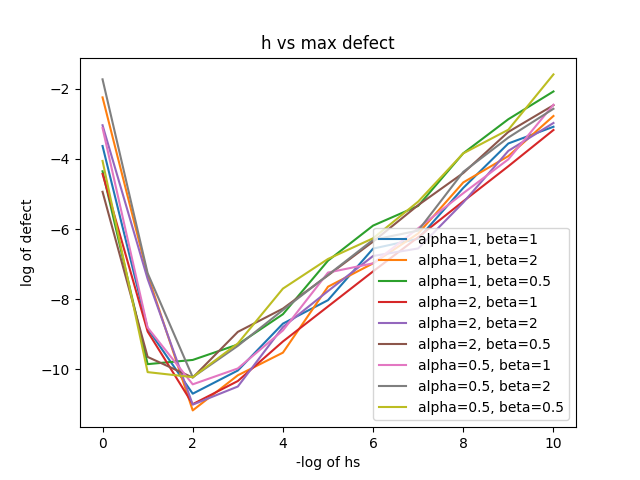
\includegraphics[width=0.7\linewidth]{./figures/future_work_hb10_v_shape}
\caption{V-shape of HB10 created by `breaking the middle step'.}
\label{fig:future_work_hb10_v_shape}
\end{figure}

\paragraph{Problems with error sampling and using a continuous L2 norm.}
================================================================
This technique is better for the error control case because we know we need a 3 point Gauss rule. i.e, if we applied it for the defect control case, we would be making 3 additional function evaluations...
Either way we can add a 'switch' in a final solver where error/defect sampling controls the maximum error/defect but 
================================================================
The shape of the error across each step is very inconsistent (See the Scaled errors plots in the previous section).One idea would be to find the max error by sampling at even more points. However, a lot of samplings would be required to reach a consistent error estimate scheme. In the next section, we present a way to sample the error using a continuous L2 norm. This essentially measures the distance between the two interpolants. By designing a continuous L2-norm scheme that maintain ratio of the error estimate from an L2 norm between two interpolants and the actual error between the interpolant and the actual solution, we guarantee that controlling the L2 norm controls the global error.

The error estimate is calculated with a continuous L2 norm as follows.
\begin{equation}
estimated\_error_i = \sqrt{ \int_{x_i}^{x_{i+1}} (\frac{h(x) - l(x)}{1 + |l(x)|})^2 \,dx }
\end{equation}
where h(x) is the higher order interpolant and l(x) is the lower order interpolant. This formula gives the error for one step and we compare it with the user provided atol for error control. 

========================
We ignored rtol as we had to factorise tol from the denominator so that we can use tol and $tol/10$ for comparisons. Essentially we assume $atol == rtol$
===================

We note that the solver performs error control through the continuous L2 norm but we want to control the actual error between the exact solution and the interpolant that was returned. To that effect, we define the following ratio: $\frac{estimated\_error_i}{exact\_error_i}$. Ideally, we want this ratio to be 1 for the scheme that we designed as a ratio of 1 entails that controlling the L2-norm would control the error between the interpolant and the exact solution.

We note that we consider the exact error is calculated with
\begin{equation}
exact\_error_i = \sqrt{ \int_{x_i}^{x_{i+1}} (\frac{sol(x) - l(x)}{1 + |l(x)|})^2 \,dx }
\end{equation}
where $sol(x)$ is the solution at point, x so that we can plot $\frac{estimated\_error_i}{exact\_error_i}$. 

To perform the integration, we use a Gauss rule. Through experimentation, we have seen that a 3-point Gauss rule was enough to produce efficient solution. A 2-point rule increased was being affected by the integration error whereas 4- and 5-points rules were not improving the number of steps taken by much showing that the integration error was no longer a limiting factor as from the 3-point rule. We note that we want to use as the smallest Gauss rule we can get away with to improve efficiency.

\subsubsection{rk4 with hb4 vs hb6 with continuous L2 norm}
Because we do not differentiate and that hb4 has order 4, we can use with rk4 with HB4 for error control. Thus HB4 and HB6 should not suffer from much interpolation error and we can use rk4 with the hb4 and hb6 using the error scheme


\paragraph{Problem 1} Figures $\ref{fig:rk4_with_hb4_hb6_L2norm_p1_global_error}$ and $\ref{fig:rk4_with_hb4_hb6_L2norm_p1_error_ratio}$ shows the global error and the ratio $\frac{estimated\_error_i}{exact\_error_i}$ on each step of using rk4 with hb4 vs hb6 with continuous L2 norm on Problem 1 at an absolute tolerance of $10^{-6}$. From Figure $\ref{fig:rk4_with_hb4_hb6_L2norm_p1_error_ratio}$, we can see that the ratio is relatively close to 1 and we can see in Figure  $\ref{fig:rk4_with_hb4_hb6_L2norm_p1_global_error}$ that the exact error is within the tolerance even when the continuous L2 norm between the two interpolant was used to control the error.

\begin{figure}[H]
\centering
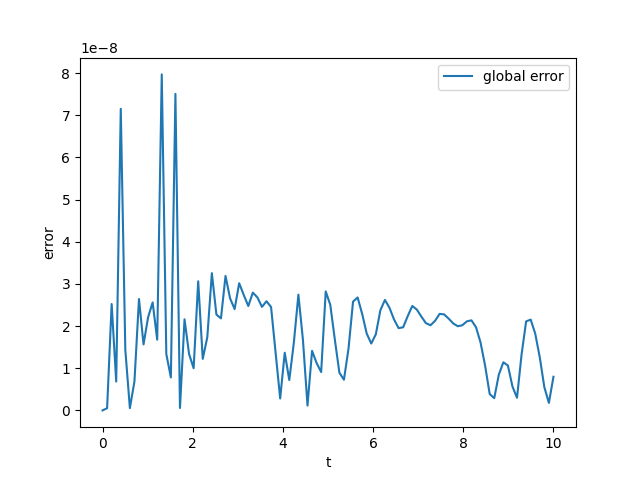
\includegraphics[width=0.7\linewidth]{./figures/rk4_with_hb4_hb6_L2norm_p1_global_error}
\caption{Global Error for RK4 with HB4 vs HB6 with continuous L2 norm on problem 1 at an absolute tolerance of $10^{-6}$.}
\label{fig:rk4_with_hb4_hb6_L2norm_p1_global_error}
\end{figure}

\begin{figure}[H]
\centering
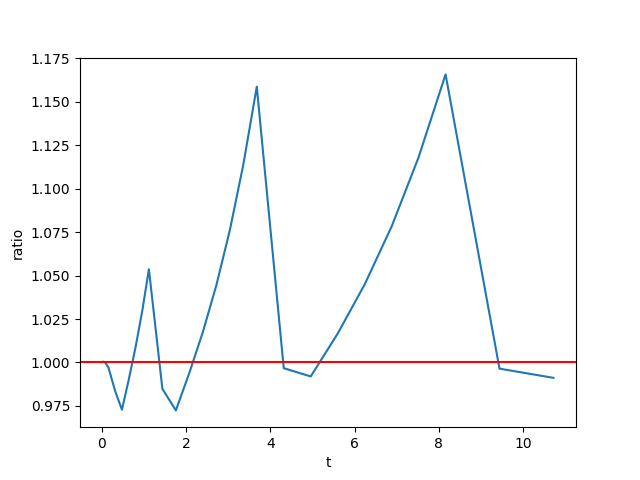
\includegraphics[width=0.7\linewidth]{./figures/rk4_with_hb4_hb6_L2norm_p1_error_ratio}
\caption{Ratio $\frac{estimated\_error_i}{exact\_error_i}$ at the end of each successful step for RK4 with HB4 vs HB6 with continuous L2 norm on problem 1 at an absolute tolerance of $10^{-6}$.}
\label{fig:rk4_with_hb4_hb6_L2norm_p1_error_ratio}
\end{figure}

\paragraph{Problem 2} Figures $\ref{fig:rk4_with_hb4_hb6_L2norm_p2_global_error}$ and $\ref{fig:rk4_with_hb4_hb6_L2norm_p2_error_ratio}$ shows the global error and the ratio $\frac{estimated\_error_i}{exact\_error_i}$ on each step of using rk4 with hb4 vs hb6 with continuous L2 norm on Problem 2 at an absolute tolerance of $10^{-6}$. From Figure $\ref{fig:rk4_with_hb4_hb6_L2norm_p2_error_ratio}$, we can see that the ratio is not relatively close to 1 and we can see in Figure $\ref{fig:rk4_with_hb4_hb6_L2norm_p2_global_error}$ that the exact error is not within the tolerance.

\begin{figure}[H]
\centering
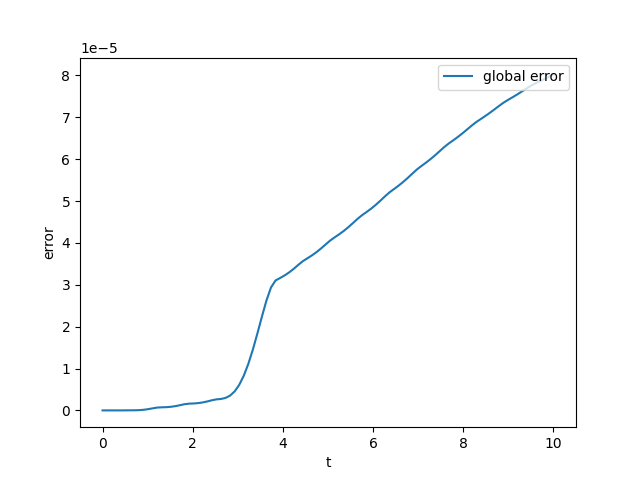
\includegraphics[width=0.7\linewidth]{./figures/rk4_with_hb4_hb6_L2norm_p2_global_error}
\caption{Global Error for RK4 with HB4 vs HB6 with continuous L2 norm on problem 2 at an absolute tolerance of $10^{-6}$.}
\label{fig:rk4_with_hb4_hb6_L2norm_p2_global_error}
\end{figure}

\begin{figure}[H]
\centering
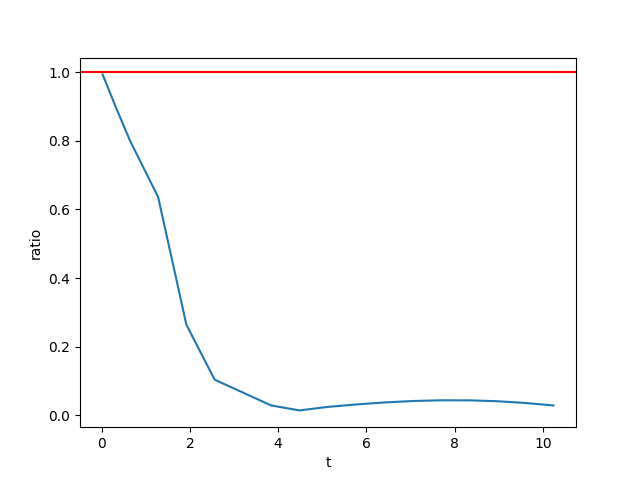
\includegraphics[width=0.7\linewidth]{./figures/rk4_with_hb4_hb6_L2norm_p2_error_ratio}
\caption{Ratio $\frac{estimated\_error_i}{exact\_error_i}$ at the end of each successful step for RK4 with HB4 vs HB6 with continuous L2 norm on problem 2 at an absolute tolerance of $10^{-6}$.}
\label{fig:rk4_with_hb4_hb6_L2norm_p2_error_ratio}
\end{figure}

\paragraph{Problem 3} Figures $\ref{fig:rk4_with_hb4_hb6_L2norm_p3_global_error}$ and $\ref{fig:rk4_with_hb4_hb6_L2norm_p3_error_ratio}$ shows the global error and the ratio $\frac{estimated\_error_i}{exact\_error_i}$ on each step of using rk4 with hb4 vs hb6 with continuous L2 norm on Problem 3 at an absolute tolerance of $10^{-6}$. From Figure $\ref{fig:rk4_with_hb4_hb6_L2norm_p3_error_ratio}$, we can see that the ratio is relatively close to 1 and we can see in Figure  $\ref{fig:rk4_with_hb4_hb6_L2norm_p3_global_error}$ that the exact error is within the tolerance even when the continuous L2 norm between the two interpolant was used to control the error.

\begin{figure}[H]
\centering
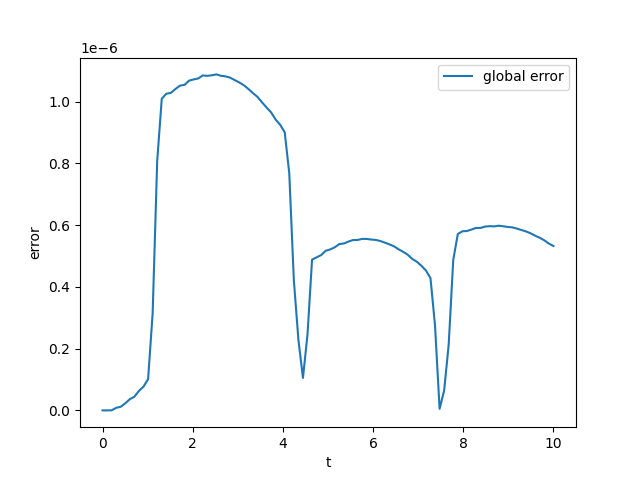
\includegraphics[width=0.7\linewidth]{./figures/rk4_with_hb4_hb6_L2norm_p3_global_error}
\caption{Global Error for RK4 with HB4 vs HB6 with continuous L2 norm on problem 3 at an absolute tolerance of $10^{-6}$.}
\label{fig:rk4_with_hb4_hb6_L2norm_p3_global_error}
\end{figure}

\begin{figure}[H]
\centering
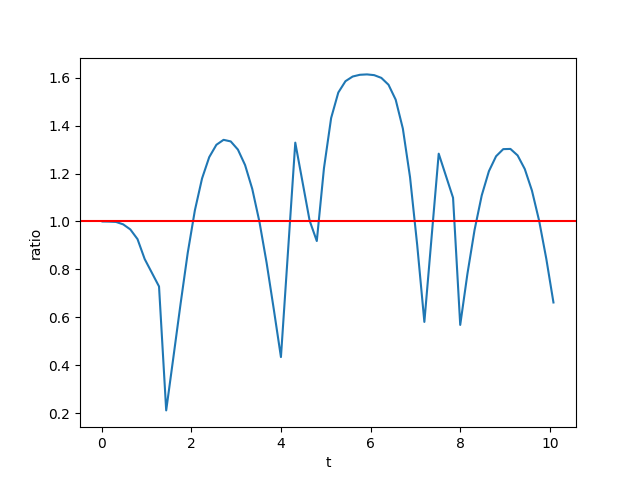
\includegraphics[width=0.7\linewidth]{./figures/rk4_with_hb4_hb6_L2norm_p3_error_ratio}
\caption{Ratio $\frac{estimated\_error_i}{exact\_error_i}$ at the end of each successful step for RK4 with HB4 vs HB6 with continuous L2 norm on problem 3 at an absolute tolerance of $10^{-6}$.}
\label{fig:rk4_with_hb4_hb6_L2norm_p3_error_ratio}
\end{figure}

\begin{table}[h]
\caption {Number of steps taken by RK4 using error control with HB4 vs HB6 by using a continuous L2 norm.} \label{tab:rk4_with_hb4_hb6_L2norm_nsteps}
\begin{center}
\begin{tabular}{ c c c } 
Problem & successful steps & total steps \\ 
1       & 27                         & 29 \\ 
2       & 20                         & 21 \\
3       & 61                         & 68 \\
\end{tabular}
\end{center}
\end{table}

\subsubsection{rk4 with hb6 vs hb8 with continuous L2 norm}
rk4 can also be use with hb6  and hb8 and not suffer from much interpolation error.



\paragraph{Problem 1} Figures $\ref{fig:rk4_with_hb6_hb8_L2norm_p1_global_error}$ and $\ref{fig:rk4_with_hb6_hb8_L2norm_p1_error_ratio}$ shows the global error and the ratio $\frac{estimated\_error_i}{exact\_error_i}$ on each step of using rk4 with hb6 vs hb8 with continuous L2 norm on Problem 1 at an absolute tolerance of $10^{-6}$. From Figure $\ref{fig:rk4_with_hb6_hb8_L2norm_p1_error_ratio}$, we can see that the ratio is relatively close to 1 and we can see in Figure  $\ref{fig:rk4_with_hb6_hb8_L2norm_p1_global_error}$ that the exact error is within the tolerance even when the continuous L2 norm between the two interpolant was used to control the error.

\begin{figure}[H]
\centering
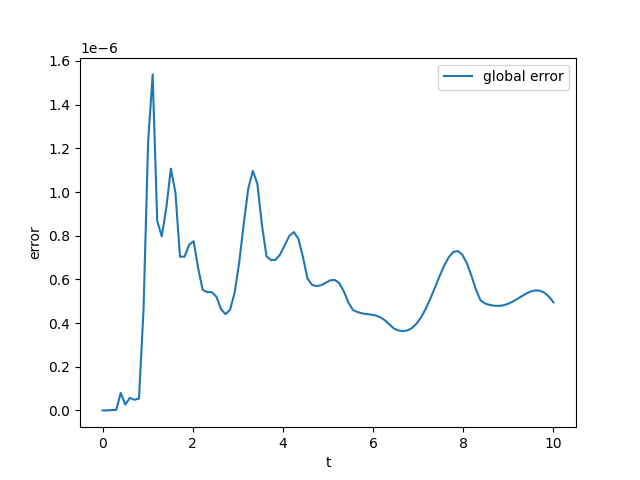
\includegraphics[width=0.7\linewidth]{./figures/rk4_with_hb6_hb8_L2norm_p1_global_error}
\caption{Global Error for RK4 with HB6 vs HB8 with continuous L2 norm on problem 1 at an absolute tolerance of $10^{-6}$.}
\label{fig:rk4_with_hb6_hb8_L2norm_p1_global_error}
\end{figure}

\begin{figure}[H]
\centering
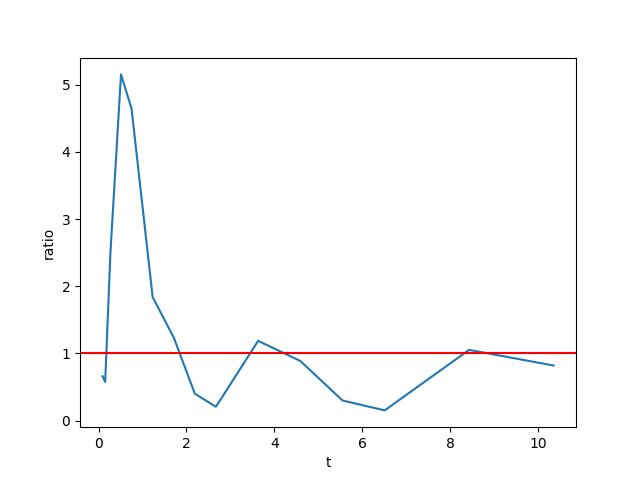
\includegraphics[width=0.7\linewidth]{./figures/rk4_with_hb6_hb8_L2norm_p1_error_ratio}
\caption{Ratio $\frac{estimated\_error_i}{exact\_error_i}$ at the end of each successful step for RK4 with HB6 vs HB8 with continuous L2 norm on problem 1 at an absolute tolerance of $10^{-6}$.}
\label{fig:rk4_with_hb6_hb8_L2norm_p1_error_ratio}
\end{figure}

\paragraph{Problem 2} Figures $\ref{fig:rk4_with_hb6_hb8_L2norm_p2_global_error}$ and $\ref{fig:rk4_with_hb6_hb8_L2norm_p2_error_ratio}$ shows the global error and the ratio $\frac{estimated\_error_i}{exact\_error_i}$ on each step of using rk4 with hb6 vs hb8 with continuous L2 norm on Problem 2 at an absolute tolerance of $10^{-6}$. From Figure $\ref{fig:rk4_with_hb6_hb8_L2norm_p2_error_ratio}$, we can see that the ratio is not relatively close to 1 and we can see in Figure $\ref{fig:rk4_with_hb6_hb8_L2norm_p2_global_error}$ that the exact error is not within the tolerance.

\begin{figure}[H]
\centering
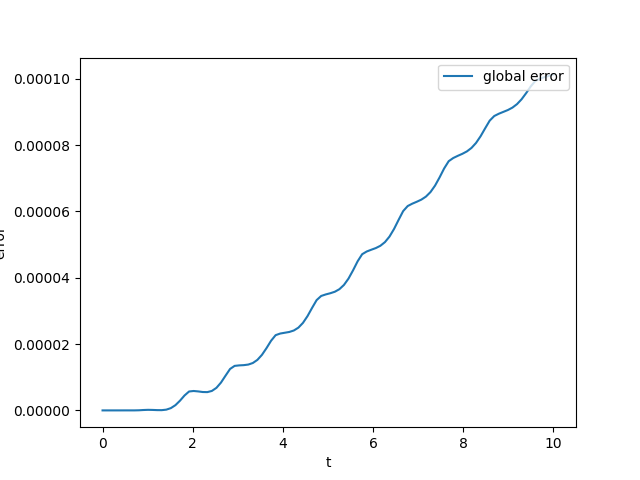
\includegraphics[width=0.7\linewidth]{./figures/rk4_with_hb6_hb8_L2norm_p2_global_error}
\caption{Global Error for RK4 with HB6 vs HB8 with continuous L2 norm on problem 2 at an absolute tolerance of $10^{-6}$.}
\label{fig:rk4_with_hb6_hb8_L2norm_p2_global_error}
\end{figure}

\begin{figure}[H]
\centering
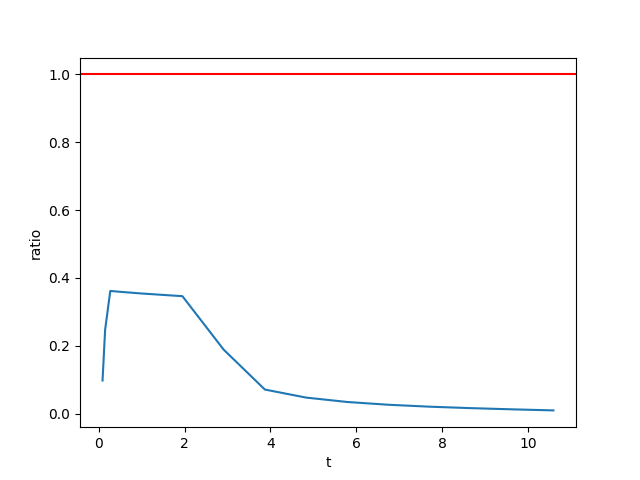
\includegraphics[width=0.7\linewidth]{./figures/rk4_with_hb6_hb8_L2norm_p2_error_ratio}
\caption{Ratio $\frac{estimated\_error_i}{exact\_error_i}$ at the end of each successful step for RK4 with HB6 vs HB8 with continuous L2 norm on problem 2 at an absolute tolerance of $10^{-6}$.}
\label{fig:rk4_with_hb6_hb8_L2norm_p2_error_ratio}
\end{figure}

\paragraph{Problem 3} Figures $\ref{fig:rk4_with_hb6_hb8_L2norm_p3_global_error}$ and $\ref{fig:rk4_with_hb6_hb8_L2norm_p3_error_ratio}$ shows the global error and the ratio $\frac{estimated\_error_i}{exact\_error_i}$ on each step of using rk4 with hb6 vs hb8 with continuous L2 norm on Problem 3 at an absolute tolerance of $10^{-6}$. From Figure $\ref{fig:rk4_with_hb6_hb8_L2norm_p3_error_ratio}$, we can see that the ratio is not relatively close to 1 and we can see in Figure $\ref{fig:rk4_with_hb6_hb8_L2norm_p3_global_error}$ that the exact error is not within the tolerance.


\begin{figure}[H]
\centering
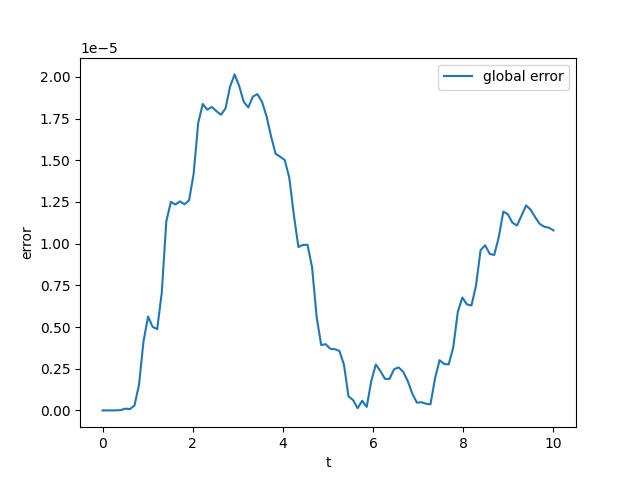
\includegraphics[width=0.7\linewidth]{./figures/rk4_with_hb6_hb8_L2norm_p3_global_error}
\caption{Global Error for RK4 with HB6 vs HB8 with continuous L2 norm on problem 3 at an absolute tolerance of $10^{-6}$.}
\label{fig:rk4_with_hb6_hb8_L2norm_p3_global_error}
\end{figure}

\begin{figure}[H]
\centering
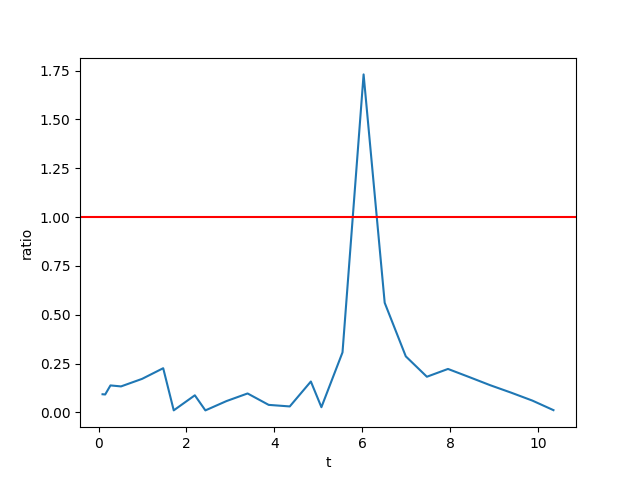
\includegraphics[width=0.7\linewidth]{./figures/rk4_with_hb6_hb8_L2norm_p3_error_ratio}
\caption{Ratio $\frac{estimated\_error_i}{exact\_error_i}$ at the end of each successful step for RK4 with HB6 vs HB8 with continuous L2 norm on problem 3 at an absolute tolerance of $10^{-6}$.}
\label{fig:rk4_with_hb6_hb8_L2norm_p3_error_ratio}
\end{figure}

\begin{table}[h]
\caption {Number of steps taken by RK4 using error control with HB6 vs HB8 by using a continuous L2 norm.} \label{tab:rk4_with_hb6_hb8_L2norm_nsteps}
\begin{center}
\begin{tabular}{ c c c } 
Problem & successful steps & total steps \\ 
1       & 15                         & 16 \\ 
2       & 15                         & 15 \\
3       & 26                         & 29 \\
\end{tabular}
\end{center}
\end{table}


\subsubsection{rk6 with hb6 vs hb8 with continuous L2 norm}
Because we do not differentiate and that hb6 has order 6, we can use with rk6 with HB6 for error control. Thus HB6 and HB8 should not suffer from much interpolation error and we can use rk6 with the hb4 and hb6 using the error scheme.

\paragraph{Problem 1} Figures $\ref{fig:rk6_with_hb6_hb8_L2norm_p1_global_error}$ and $\ref{fig:rk6_with_hb6_hb8_L2norm_p1_error_ratio}$ shows the global error and the ratio $\frac{estimated\_error_i}{exact\_error_i}$ on each step of using rk6 with hb6 vs hb8 with continuous L2 norm on Problem 1 at an absolute tolerance of $10^{-6}$. From Figure $\ref{fig:rk6_with_hb6_hb8_L2norm_p1_error_ratio}$, we can see that the ratio is relatively close to 1 and we can see in Figure $\ref{fig:rk6_with_hb6_hb8_L2norm_p1_global_error}$ that the exact error is within the tolerance even when the continuous L2 norm between the two interpolant was used to control the error.

\begin{figure}[H]
\centering
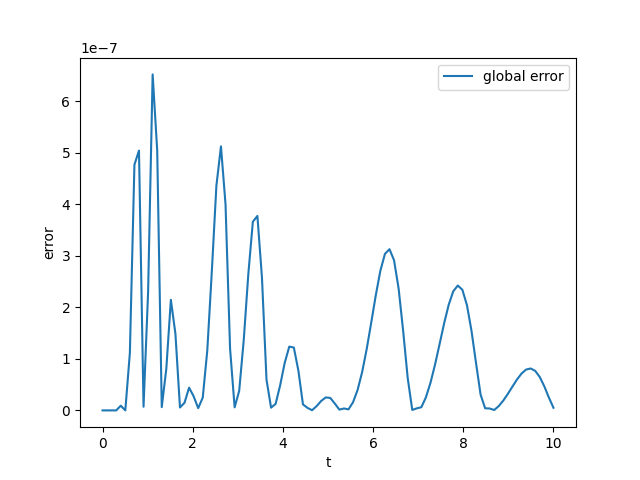
\includegraphics[width=0.7\linewidth]{./figures/rk6_with_hb6_hb8_L2norm_p1_global_error}
\caption{Global Error for RK6 with HB6 vs HB8 with continuous L2 norm on problem 1 at an absolute tolerance of $10^{-6}$.}
\label{fig:rk6_with_hb6_hb8_L2norm_p1_global_error}
\end{figure}

\begin{figure}[H]
\centering
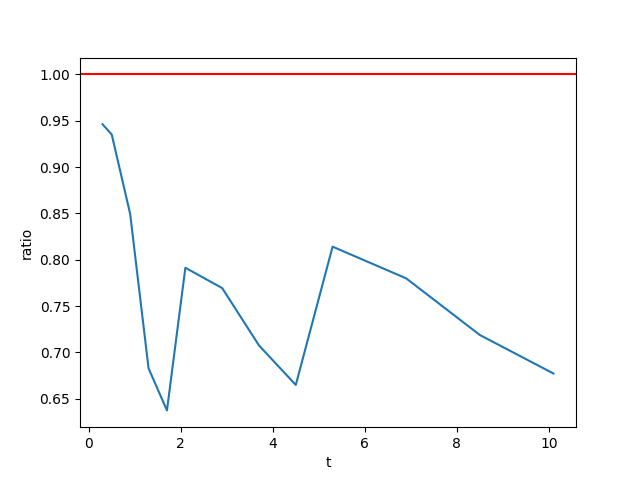
\includegraphics[width=0.7\linewidth]{./figures/rk6_with_hb6_hb8_L2norm_p1_error_ratio}
\caption{Ratio $\frac{estimated\_error_i}{exact\_error_i}$ at the end of each successful step for RK6 with HB6 vs HB8 with continuous L2 norm on problem 1 at an absolute tolerance of $10^{-6}$.}
\label{fig:rk6_with_hb6_hb8_L2norm_p1_error_ratio}
\end{figure}

\paragraph{Problem 2} Figures $\ref{fig:rk6_with_hb6_hb8_L2norm_p2_global_error}$ and $\ref{fig:rk6_with_hb6_hb8_L2norm_p2_error_ratio}$ shows the global error and the ratio $\frac{estimated\_error_i}{exact\_error_i}$ on each step of using rk6 with hb6 vs hb8 with continuous L2 norm on Problem 2 at an absolute tolerance of $10^{-6}$. From Figure $\ref{fig:rk6_with_hb6_hb8_L2norm_p2_error_ratio}$, we can see that the ratio is relatively close to 1 and we can see in Figure $\ref{fig:rk6_with_hb6_hb8_L2norm_p2_global_error}$ that the exact error is within the tolerance even when the continuous L2 norm between the two interpolant was used to control the error.

\begin{figure}[H]
\centering
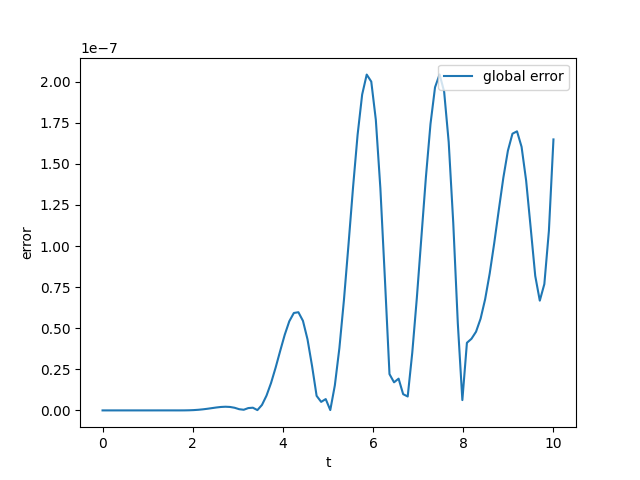
\includegraphics[width=0.7\linewidth]{./figures/rk6_with_hb6_hb8_L2norm_p2_global_error}
\caption{Global Error for RK6 with HB6 vs HB8 with continuous L2 norm on problem 2 at an absolute tolerance of $10^{-6}$.}
\label{fig:rk6_with_hb6_hb8_L2norm_p2_global_error}
\end{figure}

\begin{figure}[H]
\centering
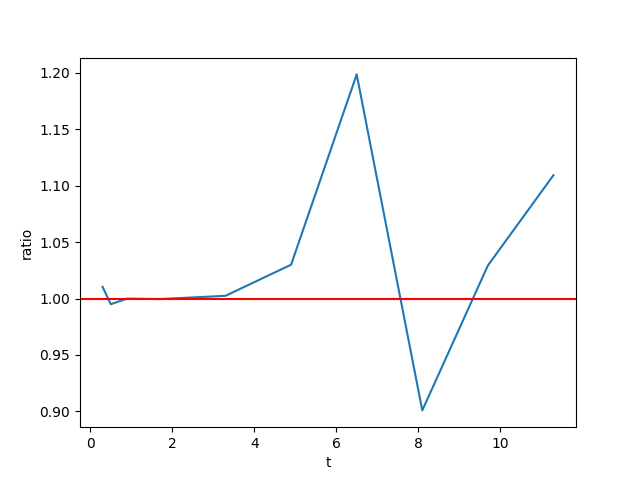
\includegraphics[width=0.7\linewidth]{./figures/rk6_with_hb6_hb8_L2norm_p2_error_ratio}
\caption{Ratio $\frac{estimated\_error_i}{exact\_error_i}$ at the end of each successful step for RK6 with HB6 vs HB8 with continuous L2 norm on problem 2 at an absolute tolerance of $10^{-6}$.}
\label{fig:rk6_with_hb6_hb8_L2norm_p2_error_ratio}
\end{figure}

\paragraph{Problem 3} Figures $\ref{fig:rk6_with_hb6_hb8_L2norm_p3_global_error}$ and $\ref{fig:rk6_with_hb6_hb8_L2norm_p3_error_ratio}$ shows the global error and the ratio $\frac{estimated\_error_i}{exact\_error_i}$ on each step of using rk6 with hb6 vs hb8 with continuous L2 norm on Problem 3 at an absolute tolerance of $10^{-6}$. From Figure $\ref{fig:rk6_with_hb6_hb8_L2norm_p3_error_ratio}$, we can see that the ratio is relatively close to 1 and we can see in Figure $\ref{fig:rk6_with_hb6_hb8_L2norm_p3_global_error}$ that the exact error is within the tolerance even when the continuous L2 norm between the two interpolant was used to control the error.


\begin{figure}[H]
\centering
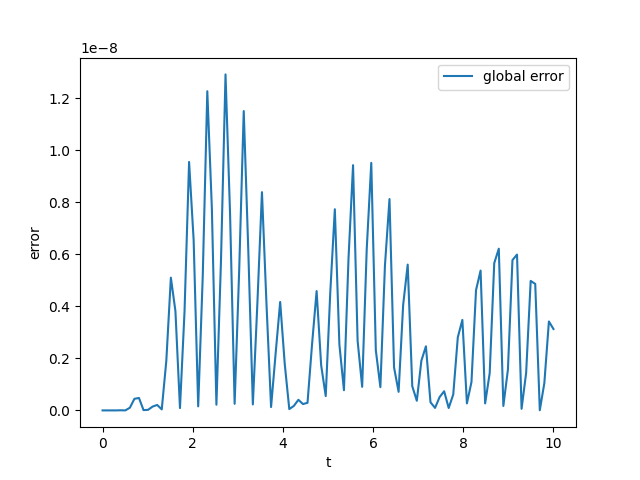
\includegraphics[width=0.7\linewidth]{./figures/rk6_with_hb6_hb8_L2norm_p3_global_error}
\caption{Global Error for RK6 with HB6 vs HB8 with continuous L2 norm on problem 3 at an absolute tolerance of $10^{-6}$.}
\label{fig:rk6_with_hb6_hb8_L2norm_p3_global_error}
\end{figure}

\begin{figure}[H]
\centering
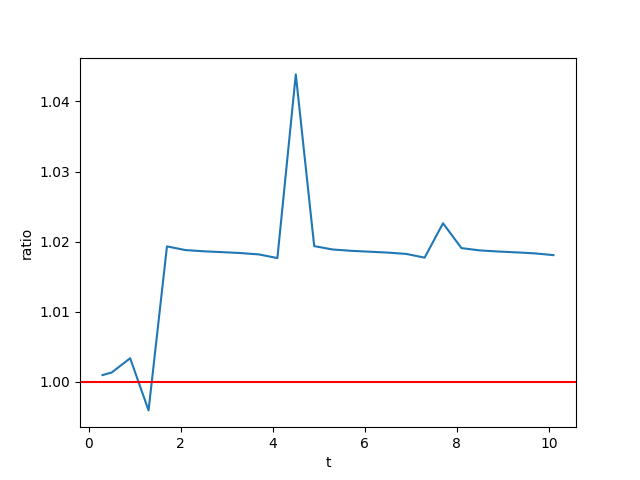
\includegraphics[width=0.7\linewidth]{./figures/rk6_with_hb6_hb8_L2norm_p3_error_ratio}
\caption{Ratio $\frac{estimated\_error_i}{exact\_error_i}$ at the end of each successful step for RK6 with HB6 vs HB8 with continuous L2 norm on problem 3 at an absolute tolerance of $10^{-6}$.}
\label{fig:rk6_with_hb6_hb8_L2norm_p3_error_ratio}
\end{figure}

\begin{table}[h]
\caption {Number of steps taken by RK6 using error control with HB6 vs HB8 by using a continuous L2 norm.} \label{tab:rk6_with_hb6_hb8_L2norm_nsteps}
\begin{center}
\begin{tabular}{ c c c } 
Problem & successful steps & total steps \\ 
1       & 13                         & 15 \\ 
2       & 10                         & 10 \\
3       & 26                         & 36 \\
\end{tabular}
\end{center}
\end{table}